\begin{frame}
  \frametitle{Introduction}
  % a comment
        \begin{columns}
                \column[t]{5cm}
                \begin{itemize}
                \item Foucs on modeling the fuel circuit of the \gls{MSFR} duirng transients. 

                \item Neutronics and thermal hydraulics are strongly coupled  

                \item Model the coupling during transients: RIA and load following  

                \item Reference reactor configuration:
                \begin{itemize}
                        \item 3 GWth liquid fueled reactor
                        \item Salt volume of 18 m$^3$
                        \item Salt average temperature of 975 K
                        \item Salt is 75\% LiF, 25\% HMF (mix of Th and fissile material)
                        \item Salt circulation time is 4 s
                \end{itemize}
                \end{itemize}
                
                \column[t]{5cm}
                \begin{figure}[htbp!]
                        \begin{center}
                        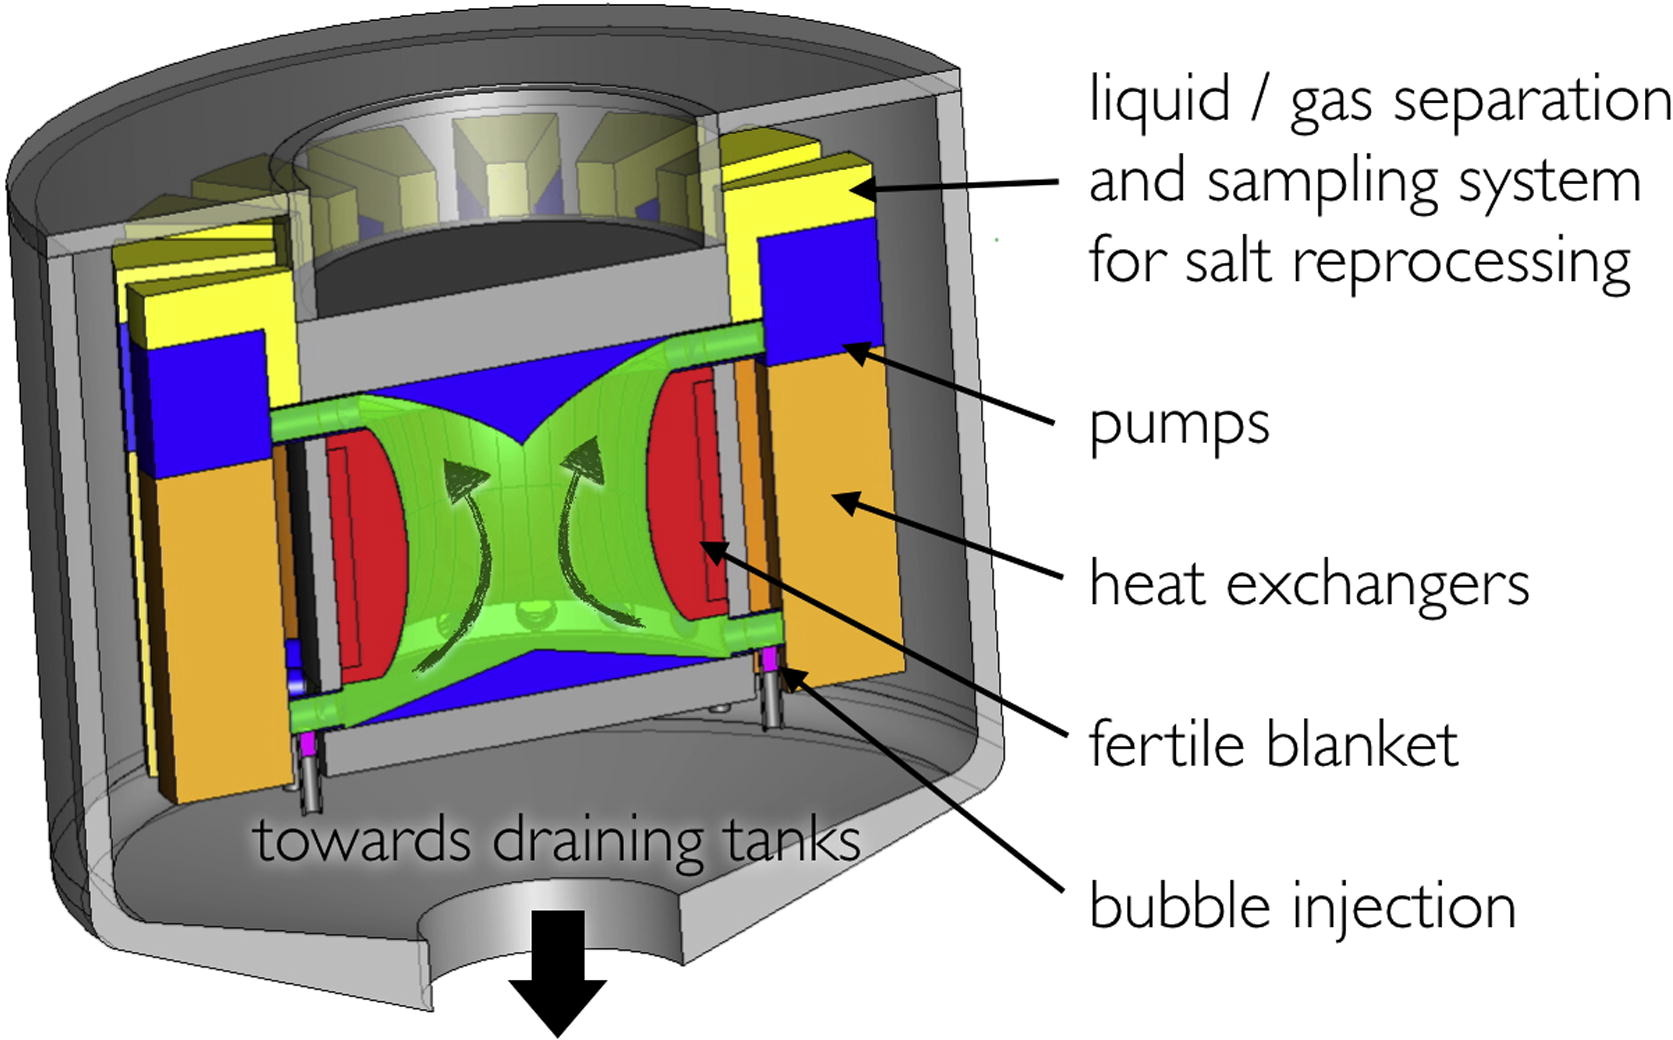
\includegraphics[scale=0.65]{JC-Oct16/reactor-loops.jpg}
                        \end{center}
                        \caption{\gls{MSFR} circuit configuration}
                        \label{fig:MSFR circuit}
                \end{figure}
        \end{columns}
\end{frame}

\begin{frame}
  \frametitle{Methodology}
  %\begin{columns}
   %     \column[t]{5cm}
        Couple neuronics and thermal hyrdaulics using a Transient Fission Matrix (TFM)
        in Serpent and the CFD code OpenFOAM
        \begin{itemize}
                \item TFM contain the transport of neutrons during a generation in a spatially discretized reactor with a temporal aspect
                \item Used a modified Serpent code to calculate the TFM
                \item Used Reynolds-Averaged Navier Stokes approach for TH

        \end{itemize}

    %    \column[t]{5cm}
        \begin{figure}
                \centering
                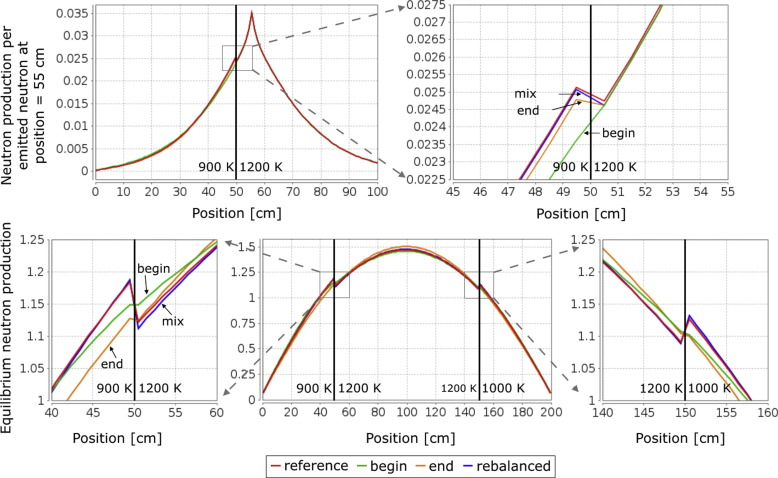
\includegraphics[scale=0.5]{JC-Oct16/neutron-matrix.jpg}
                \label{fig:matrix}
        \end{figure}

  %\end{columns}
\end{frame}


\begin{frame}
  \frametitle{Validation}
  First had to couple the two components
        \begin{itemize}
                \item Serpent is used to calculate the TFM, prior to transients
                \item Integrate precursor calculation into TH source code     
        \end{itemize}
  Used reference case using direct Serpent and OpenFOAM coupling previously defined

 
  \begin{figure}
        \centering
        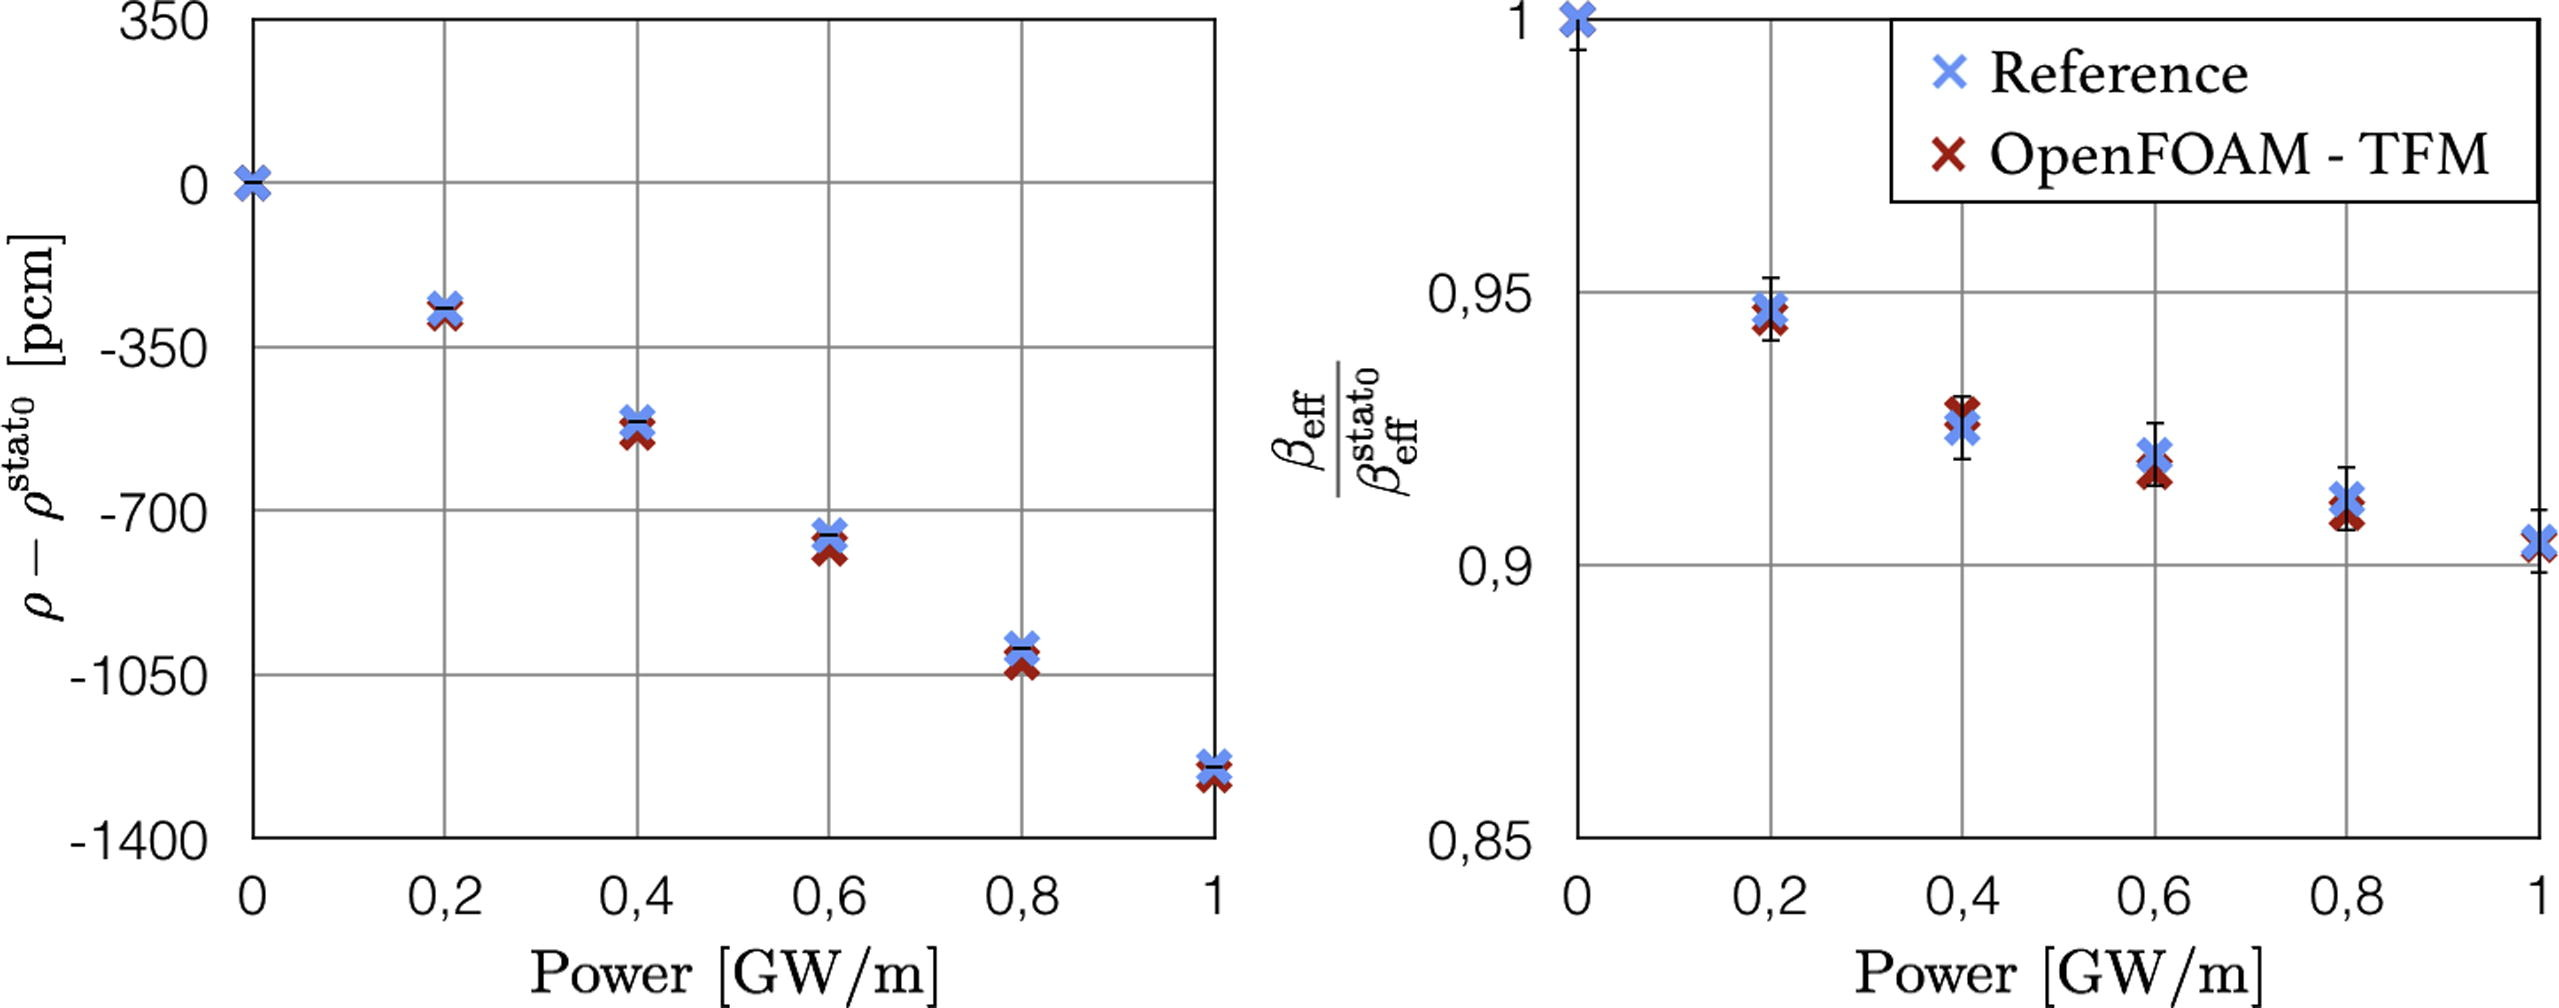
\includegraphics[scale=0.65]{JC-Oct16/reference.jpg}
        \label{fig:reference}
  \end{figure}
              
\end{frame}
